\chapter{Variance}

\section{Introduction}

\begin{figure}
\centering
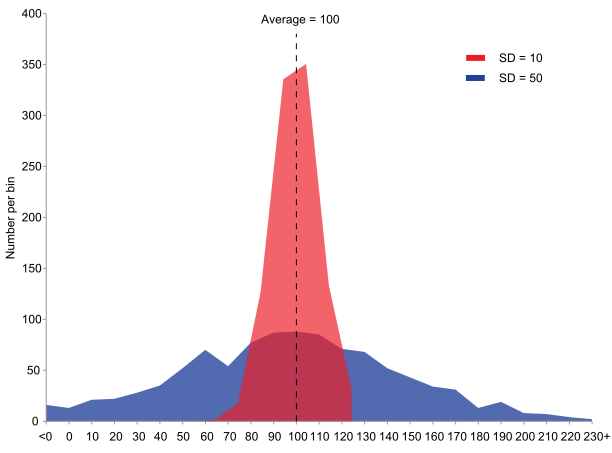
\includegraphics[width=0.9 \textwidth]{Comparison_standard_deviations}
\caption{Example of samples from two populations with the same mean
  but different variances. The red population has mean 100 and
  variance 100 (SD=10) while the blue population has mean 100 and
  variance 2500 (SD=50) where SD stands for Standard Deviation.}
\end{figure}

In probability theory and statistics, \textbf{variance} is the
expected value of the squared deviation from the mean of a random
variable. The standard deviation (SD) is obtained as the square root
of the variance. Variance is a measure of dispersion, meaning it is a
measure of how far a set of numbers is spread out from their average
value. It is the second central moment of a distribution, and the
covariance of the random variable with itself, and it is often
represented by $\sigma^2$, $s^2$, $\operatorname{Var}(X)$, $V(X)$, or
$\mathbb{V}(X)$.

An advantage of variance as a measure of dispersion is that it is more
amenable to algebraic manipulation than other measures of dispersion
such as the expected absolute deviation; for example, the variance of
a sum of uncorrelated random variables is equal to the sum of their
variances. A disadvantage of the variance for practical applications
is that, unlike the standard deviation, its units differ from the
random variable, which is why the standard deviation is more commonly
reported as a measure of dispersion once the calculation is finished.

There are two distinct concepts that are both called
``variance''. One, as discussed above, is part of a theoretical
probability distribution and is defined by an equation. The other
variance is a characteristic of a set of observations. When variance
is calculated from observations, those observations are typically
measured from a real-world system. If all possible observations of the
system are present, then the calculated variance is called the
population variance. Normally, however, only a subset is available,
and the variance calculated from this is called the sample
variance. The variance calculated from a sample is considered an
estimate of the full population variance. There are multiple ways to
calculate an estimate of the population variance, as discussed in the
section below.

The two kinds of variance are closely related. To see how, consider
that a theoretical probability distribution can be used as a generator
of hypothetical observations. If an infinite number of observations
are generated using a distribution, then the sample variance
calculated from that infinite set will match the value calculated
using the distribution's equation for variance. Variance has a central
role in statistics, where some ideas that use it include descriptive
statistics, statistical inference, hypothesis testing, goodness of
fit, and Monte Carlo sampling.


\subsection{Definition}\label{definition}

The variance of a random variable $X$ is the expected value of the
squared deviation from the mean of $X$, $\mu = \operatorname{E}[X]$:
$$\operatorname{Var}(X) = \operatorname{E}\left[(X - \mu)^2 \right].$$

This definition encompasses random variables that are generated by
processes that are discrete, continuous, neither, or mixed. The
variance can also be thought of as the covariance of a random variable
with itself:
$$\operatorname{Var}(X) = \operatorname{Cov}(X, X).$$

The variance is also equivalent to the second cumulant of a
probability distribution that generates $X$. The variance is typically
designated as $\operatorname{Var}(X)$, or sometimes as $V(X)$ or
$\mathbb{V}(X)$, or symbolically as $\sigma^2_X$ or simply
$\sigma^2$ (pronounced ``sigma squared''). The expression for the
variance can be expanded as follows:
\begin{align*}
\operatorname{Var}(X) &= \operatorname{E}\left[(X - \operatorname{E}[X])^2\right] \\
&= \operatorname{E}\left[X^2 - 2X\operatorname{E}[X] + \operatorname{E}[X]^2\right] \\
&= \operatorname{E}\left[X^2\right] - 2\operatorname{E}[X]\operatorname{E}[X] + \operatorname{E}[X]^2 \\
&= \operatorname{E}\left[X^2 \right] - \operatorname{E}[X]^2
\end{align*}

In other words, the variance of $X$ is equal to the mean of the square of $X$
minus the square of the mean of $X$. This equation should not be used for
computations using floating point
arithmetic, because it suffers from catastrophic cancellation if the two
components of the equation are similar in magnitude. 

[\ldots Original Wikipedia article continues \ldots]

\subsubsection{Commonly used probability
distributions}\label{commonly_used_probability_distributions}

Table \ref{tab:var_dist} lists the variance for some commonly used
probability distributions.

\begin{table}[h]
\begin{tabular}{@{}llll@{}}
\toprule
Name  & Probability distribution function
& Mean & Variance \\
\midrule
Binomial distribution & $\Pr\,(X=k) = \binom{n}{k}p^k(1 - p)^{n-k}$ & $np$ & $np(1 - p)$ \\
Geometric distribution & $\Pr\,(X=k) = (1 - p)^{k-1}p$ & $\frac{1}{p}$ & $\frac{(1 - p)}{p^2}$ \\
Normal distribution &
$f\left(x \mid \mu, \sigma^2\right) = \frac{1}{\sqrt{2\pi\sigma^2}} e^{-\frac{(x - \mu)^2}{2\sigma^2}}$
& $\mu$ & $\sigma^2$ \\
Uniform distribution &
$f(x \mid a, b) = \begin{cases}
  \frac{1}{b - a} & \text{for } a \le x \le b, \\[3pt]
                0 & \text{for } x < a \text{ or } x > b
\end{cases}$ & $\frac{a + b}{2}$ & $\frac{(b - a)^2}{12}$ \\
Exponential distribution &
$f(x \mid \lambda) = \lambda e^{-\lambda x}$ & $\frac{1}{\lambda}$ &
$\frac{1}{\lambda^2}$ \\
Poisson distribution &
$f(k \mid \lambda) = \frac{e^{-\lambda}\lambda^{k}}{k!}$ & $\lambda$
  & $\lambda$ \\
  \bottomrule
\end{tabular}
\caption{\label{tab:var_dist} Basic properties of some commonly used probability distributions.}
\end{table}

\subsection{Properties}\label{properties}

\subsubsection{Basic properties}\label{basic_properties}

[This section is altered from to the original Wikipedia
  article to try out the AMS theorem environments.]

\begin{theorem}
  The variance  of any random variable $X$ is non-negative
  $$\operatorname{Var}(X)\ge 0.$$
\end{theorem}

\begin{proof}
  Since $(X - \mu)^2 \geq 0$,
  \[\operatorname{Var}(X) = \operatorname{E}\left[(X - \mu)^2\right] \geq 0.\]
\end{proof}

[Original Wikipedia article continues \ldots]
